\section{August - November 2011}
\subsection*{2011-08-15 Treffen mit Oliver/Karen}

\begin{figure}[h]
	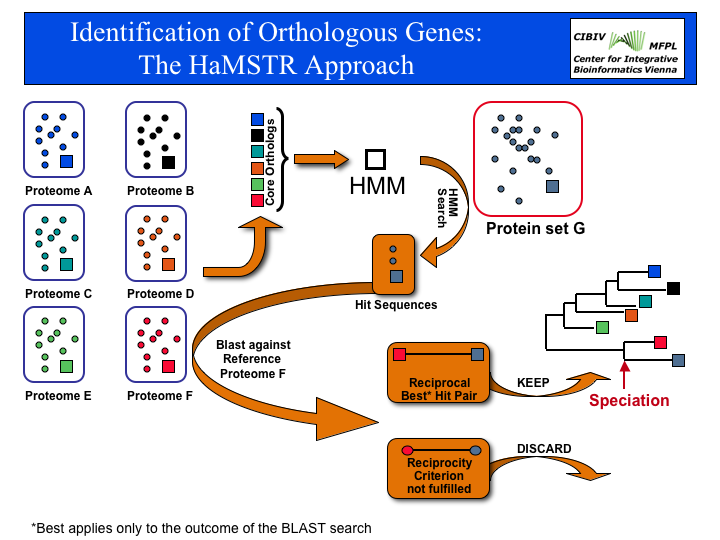
\includegraphics[width=\textwidth]{img/hamstr-schema}
	\caption{\cite{Ebersberger2009}}
\end{figure}

Tasks:

\begin{itemize}
	\item read paper
	\item install HaMStR, test
	\item read \& understand the source:
		\begin{itemize}
			\item what is happening when
			\item at what point does it use genewise?
		\end{itemize}
	\item look up:
		\begin{itemize}
		\item genewise/exonerate (alignment NA $\rightarrow$ AA)
			\item PAL2NAL
			\item ESTwiseDB
			\item BLASTx (what does it do)
		\end{itemize}
\end{itemize}

Vortrag beim Montagskolloquium über DA (desinteressiertes, ahnungsloses
Publikum)

\begin{itemize}
	\item Warum?
\end{itemize}

\subsection*{2011-08-16}

Installed HaMStR v8 with all dependencies:

\begin{table}[h]
	\begin{tabular}{l l l}
		\textbf{Package} & \textbf{Version} & \textbf{Source}\\
		\hline
		HMMer    & 3.0	 & http://www.deep-phylogeny.org/hamstr/download/ \\
		ClustalW & 2.1   & ftp://ftp.ebi.ac.uk/pub/software/unix/wise2/ \\
		Genewise & 2.2.0 & http://hmmer.janelia.org/software \\
	\end{tabular}
\end{table}

All programs were installed in PATH. With Genewise, a modification was
neccessary in \file{src/HMMer2/sqio.c}: renamed getline() to genewise\_getline()
since getline() is already defined in \file{stdio.h} (standard C library).

All test runs according to the README files were successful.

Read the HaMStR paper (\cite{Ebersberger2009}).

Tried to get an insurance for the lab key, so far unsuccessful.

\subsection*{2011-08-17}

Picked up playground data and annotations from Karen.

\subsection*{2011-08-18 What does HaMStR do?}

Genewise: At the very end, \emph{after} the re-BLAST. Translates ESTs to
revcomp, only if at least one hit was obtained.

\subsection*{2011-08-23 Karen}

\begin{itemize}
	\item ``transitive closure'' $\rightarrow$ lookup \url{deep-phylogeny.org}
	\item InParanoid: Orthology by pairwise assignment
	\item OrthoMCL: Orthology by pairwise $\rightarrow$ groups of orthologs. Read
		presentations.
	\item parallelize: spawn daughter processes according to \#CPU?
\end{itemize}

\subsection*{2011-08-24 Oliver}

``deep search'': blast instead of hmmsearch (weniger sensitiv)

``very deep search'': hmm hits mit estwisedb (übersetzen und suchen in 1) gegen
core-orthologs

Warum nur orthologe Gene durchsuchen? $\rightarrow$ auch nicht orthologe,
vielleicht passen sie besser.

EST-Set schrittweise verkleinern\dots

Benchmarks mit absichtlich verschlechterten Sequenzen, z.B. einen von den
Core-Orthologen zufällig verändern.

\begin{table}
	\begin{tabular}{l l}
	\textbf{program} & \textbf{compares} \\
	\hline
	genewise   & single protein vs single DNA seq \\
	genewisedb & protein database vs DNA database \\
	estwise    & single protein vs single EST/cDNA seq \\
	estwisedb  & protein database vs EST/cDNA database
	\end{tabular}
\end{table}

valid command line:
\begin{verbatim}
../hamstrsearch_local-hmmer3.v8.pl
-sequence_file=cleaned/Adelphocoris_lineolatus_contig.fa
-fasta_file=ortholog_set_insecta_hmmer3-1/insecta_hmmer3-1.fa -taxon=apime
-refspec=dappu_1391 -blast_path=ortholog_set_insecta_hmmer3-1/blast_dir -est
\end{verbatim}

\section{September 2011}
\subsection*{2011-09-02}

Karen nach Erklärung fragen:
\renewcommand{\labelenumi}{\alph{enumi})}
\begin{enumerate}
	\item Frameshifts + deren Korrektur
	\item Introns + interne Stopcodons: Wie erkennen und sinnvoll entfernen?
\end{enumerate}

\includegraphics[width=0.5\textwidth]{img/hamstr-cmdline-files.pdf}
\begin{table}[h]
\begin{tabular}{l l l}
	\textcircled{A} & cleaned/Adelphocoris\_lineolatus\_contig.fa & $\leftarrow$ EST file (fasta)\\
	\textcircled{B} & ortholog\_set\_insecta\_hmmer3-1/insecta\_hmmer3-1.fa & $\leftarrow$ Core ortholog set (fasta)\\
	\textcircled{C} & dappu\_1391 & $\leftarrow$ reference taxon, from the core set \\
	 \textcircled{D} & ortholog\_set\_insecta\_hmmer3-1/blast\_dir & $\leftarrow$ BLAST database for the re-BLAST
\end{tabular}
\end{table}

\subsection*{2011-09-05 $\rightarrow$ 11 Started writing FORAGE}

\textbf{F}ind \textbf{O}rthologs using \textbf{R}eciprocity \textbf{A}mong
\textbf{G}enes and \textbf{E}STs 

\begin{description}
\item[Forage, v.:] Durchsuchen, (nach Nahrung) suchen etc.
\end{description}

There are BioPerl modules for 
\begin{enumerate}
	\item translation to all 6 reading frames
	\item using HMMer
	\item using BLAST
	\item reading \& writing files
\end{enumerate}
(but Oliver and Bernhard think I should stay away from them)

\subsection*{Intranet}

\fbox{\lstinline{boutEST\&Protein!2011}}

\begin{tabular}[h]{l l}
	\url{svzfmksql03} & $\rightarrow$ Server \\
	\url{131.220.75.253} & ~\\
	\url{lpd://131.220.75.250/przfmk010} & PPD: Apple 12/640ps\\
	\url{przfmk010} & 2. Etage\\
	\url{przfmk09} & 1. Etage\\
	\url{domzfmk} & Domain\\
	\url{131.220.228.166} & Cluster (pwd zfmk)\\
	\url{131.220.228.163} & alter Cluster\\
\end{tabular}

VPN? $\rightarrow$ Christoph fragen

\begin{lstlisting}
smbclient -W DOMZFMK -U <username> //SVZFMKSQL03/Molekular-Labor
\end{lstlisting}

\verb|mount.cifs| in \file{fstab}:
\begin{lstlisting}
//svzfmksql03/molekularlabor/ /mnt/zfmknet cifs noauto,users,credentials=/path/to/credsfile 0 0
\end{lstlisting}

\subsection*{2011-09-14}

Fiddled around with BioPerl, tried to reproduce Hamstr

hmmfound nothing in Andrena\_vaga $\rightarrow$ can this be true? Double-check!

\vspace{1em}
\begin{minipage}{0.4\textwidth}
	\begin{itemize}
		\item Substitute Unix tools w/ builtin Perl functions, e.g. grep/sed
		\item Debugging
		\item InParanoid source?
		\item CC license
		\item ``Forage''
		\item Computer?
	\end{itemize}
\end{minipage}
\hfill
\begin{minipage}{0.5\textwidth}
\textbf{PRIORITÄTEN}
\renewcommand{\labelenumi}{\arabic{enumi}.}
	\begin{enumerate}
		\item Korrigierte Nucleotide-Seq zu den Amino-Alignments die Hamstr
		ausspuckt $\rightarrow$ genewise-output speichern und parsen $\rightarrow$ pal2nal,
		sonst exonerate $\rightarrow$ Gerrit fragen! Prob?
		\item Orthologen-Set erstellen
	\end{enumerate}
\url{(arthropods.)eugenes.org}
\end{minipage}

\subsection*{2011-09-15}

be paranoid about BioPerl

\subsection*{2011-09-27 after I got this lab journal back\dots}

how the data structure could look like in Forage:

\begin{verbatim}
             {EST ID}
                 |
                 v
{seq, matched_by_hmm, hmm_score}
\end{verbatim}

how the data structure looks like in Hamstr:
\begin{verbatim}
            {taxon}
               |
               v
{prot=>hmm-hit seq, ids=>hmmhits, refseq=>refspec-seq, refspec=>refspec}
\end{verbatim}

\subsection*{2011-09-28}

\begin{lstlisting}
	$gw->{gw}	# ref to array
	print join("\n", @$gw->{gw})	# "not an ARRAY reference" error
	my $out = $gw->{gw};
	print join("\n", @$out); # works -> WTF?
\end{lstlisting}

Solution: dereferencing done correctly: 
\begin{lstlisting}
	print join("\n", @{$gw->{gw}}
\end{lstlisting}

\begin{itemize}
	\item ursprüngliche, korrigierte Nuc-Sequenz fehlt im Hamstr-output
	\item steht in genewise-output?
	\item sonst exonerate
	\item testen was genewise ausspuckt, wenn seq.\ künstlich verändert
	$\rightarrow$ frameshift, zus.\ A etc
\end{itemize}

\subsection*{2011-09-30 genewise splittet bei frameshifts}

\subsection*{2011-09-X cluster access}

\url{mptersen@131.220.228.166} pwd \url{zfmk}

List of installed software: \url{131.220.75.250}

Queueing system:

\begin{table}[h]
	\begin{tabular}{l l l}
	\verb|qsub| & <bash script> & (multiple opts for the script\dots RTFM)\\
	\verb|qstat| & show running stuff & (\verb|-f| full output)\\
	\verb|qdel| & delete jobs & ~ \\
	\verb|qhost| & show running stuff & (\verb|-j| by all users)\\
	\verb|mpirun| & for MPI & $\rightarrow$ only where it makes sense, read docs
	first!
	\end{tabular}
\end{table}

important: no relative paths in scripts

\section{October 2011}
\subsection*{2011-10-05}
\begin{verbatim}
	genewise -cdna -trans -sum -pep
\end{verbatim}
\verb|-gff| mögl.? $\rightarrow$ cdna zum pep-Alignment speichern, pal2nal

\verb|s/genewise/exonerate/ ?|

\subsection*{2011-10-18 been working on substitution of genewise by exonerate}
genewise is 
\begin{inparaenum}
	\item slower, 
	\item less able and 
	\item does not output cDNA for its translation.
\end{inparaenum}

exonerate is
\begin{inparaenum}
	\item fast,
	\item more precise (does not cut off as much as genewise if there are
	frameshifts), and 
	\item does output cDNA instead of the translation.
\end{inparaenum}

The cDNA sequences are desired.

Done so far:
\begin{itemize}
	\item reproduced genewise output in exonerate (sp, pep, sp.tr)
	\item modified run\_genewise\_hamstr.pm to run exonerate instead of genewise
	(now called exonerate.pm)
\end{itemize}

\begin{description}
\item[discoveries:] the exonerate package brings along a number of fasta-file
modification tools, including \emph{fastatranslate}, which can \emph{100\%
replace} the BioPerl translate\_6frames and is \textasciitilde 10x faster
(written in C)
\item[problems:] exonerate has no means of outputting the \# of indels - this is
used by Hamstr to determine how to concatenate the seq fragments after
translation
\item[$\rightarrow$] if there are indels, they are tr'ed to lower case, if not,
represented as 'N'
\end{description}

\section{December 2011}
\subsection*{Thu Dec  1 00:01:30 CET 2011}

Finally fixed and manicured the cdna bug in Hamstr. It now works as expected,
including corresponding cdna output. I still want to optimize the terminal
messages.

Jeanne wrote a script that creates a Hamstr-compatible core ortholog set from a
bunch of OGS FASTA files. Apart from a few bugs which may already be fixed, it
works very well already. It runs fastatranslate, muscle/mafft and hmmbuild and
takes a couple of hours. I used a newly generated ortholog set with Hymenoptera
(mostly ants) and let Hamstr chew on Andrena vaga with it, and it appears to
work very well, spits out beautifully matching sequences. 

Tanja has been working on a summarizer script that packs the Hamstr output into
human-readable form. In particular, it compiles the AA sequences of all the
hamstred taxa along with the core orthologs in one FASTA file, aligns it and
cuts out the core ortholog seqs again so that we are left with the aligned query
taxon seqs. Very nice and useful. She has been doing a lot of careful work, and
has now been provided with real-life output to test and fine-tune her script
with.

I have to start preparing the presentation for the MoKo on Dec 19th. Oliver has
given me a couple of valuable tips for structure, content and design. Will
probably do the thing in \LaTeX\ again, I am beginning to really like the beamer
package. Along with the textpos package, positioning graphics and stuff anywhere
I want is no longer a hassle. And it just looks so beautiful\ldots

\subsection*{Fri Dec  2 18:40:54 CET 2011}

Didn't do anything in Hamstr the last two days. Rather, was of assistance to
Jeanne and Tanja and had a couple of discussions with Karen/Oliver/Bernhard.
Tanja accidentally uncovered a problem when summarizing the Hamstr output: When
a sequence contains stop codons (TAA, TAG, TGA), they will be cut out/replaced
with gaps by MUSCLE or MAFFT. Therefore, and since we want them conserved, Tanja
will replace them with 'x' before the alignment step and replace them back once
the alignment is complete. MAFFT allows to preserve case, MUSCLE does not.
Tanjas Program will only use MAFFT-LINSI in the future.

I was a little surprised that nobody seemed to have given the stop codons any
thought so far. Do they carry phylogenetic information? How do they influence the
tree inference? How do they mutate, if they do at all? I'll have to look this
up. I wrote a small script to check the sequence lengths of amino acid and
nucleotide output, but they always match. Hamstr itself does nothing to the stop
codons.

Jeanne is getting bored; she needs a challenge. Even adding the nucleotide to
the newly generated core ortholog set isn't going to take her more than a day, I
think. I wonder if I could think about something that would really make her
ponder\ldots Something like the prime numbers that she would think about more
than a day. I don't know. Maybe I'll introduce her to \url{projecteuler.com}
next week.

Yesterday, Alex did his Momento talk about the new cluster. It went quite well,
but took too long, I think. 

\subsection*{Sun Dec 11 14:37:13 CET 2011}

Jeanne's and Tanja's lab module ended on Friday. They both finished the
programs they worked on, and although Karen and I didn't get a chance to test
them, they appear work fine. Well, I hope so, because none of us is going to
find the time to bug-fix or really work on them. They did leave a good
impression, though, and maybe one (or both) of them will write their master's
thesis here, as well. 

I started working on FORAGE again, too. Exchanged Path::Class for File::Spec and
re-wrote the hmmsearch output parser so that pre-existing result files are not
skipped, but their content is made available. Now everything is ready to get out
the hits and do the reciprocal search.

Tomorrow I'm flying to Vienna because they made me :) No, I'm excited what to
expect there, I've never been to a real scientific meeting before. Karen, Caro,
Bernhard and I are going to visit another work group there that is also part of
the 1KITE project (\url{1kite.org}). I'm also going to give the ten-minute talk
about HaMStR and my thesis there, which I'm also going to give the Monday after
in the MoKo. I've been polishing it for days and I think it's in a semantically
sensible structure now. I hope everybody thinks the same when I give it for real.

\subsection*{Wed Dec 14 22:27:45 CET 2011}

I just got back from Vienna and am waiting for the train home. These last few
days have been extraordinarily great for me, which is why I will allow some more
intimate thoughts in this journal tonight. 

We visited the work groups of Nicola Szucsich and Daniela Bartels at the
University of Vienna from Monday to today. We departed Cologne at 0650 (in the
morning - gah!) and landed in Vienna some one and a half hour later and took the
trains straight to the university and met that work group. These people are so
nice and friendly\ldots It has really been a pleasant surprise meeting them,
although I am normally very wary of meeting new people. Anyway, we had coffee
and then Karen spoke for over four hours about ESTs and what we do with them.
Not about Hamstr, that has been saved for Tuesday. Nicola and Dani had a lot of
questions, especially about the sequence assemblers and MARE. What puzzled them
most was the way the four competing tree topologies were not only generated, but
also scored and compared. How can there be more than one topology for a given
dataset in a ML analysis? I don't even remember\ldots that part was in the late
afternoon, and I was having a low and very nearly fell asleep during that
discussion.

In the evening, we rode to Nicola and Dani's. They live together, have a young
child and are apparently very much in love with each other. Very nice to watch,
especially seeing a university professor on his knees, in a dirty sweater, and
trying to talk his daughter into pushing a triangular brick into a triangular
hole. If anything, it only made him more human. Hannah, their daughter, was very
cool. Well, we had dinner and sat until midnight.

The next day, Bernhard arrived, and I gave my talk, which I have been polishing
thoroughly. 

\subsection*{Wed Dec 28 18:34:30 CET 2011}

Didn't finish reporting about Vienna -- nevermind. 

I got back to FORAGE the last few days before Christmas. The Forage::Item module
is now fully object-oriented, the class abstraction layer is complete. No more
direct access to the object data like in Hamstr :P 

In the new year, I can't wait to get to the reciprocal search part. I did some
performance test and found out the following:

\begin{description}
	\item[open, while readline] seems to be the fastest way of finding
	a certain string in a file. 
	\item[open, read into array, grep] is slower, and requires more memory.
	\item[Tie::File] is awfully slow.
	\item[system calls to grep] are also very fast, but probably have more
	overhead because of the system call, and add to platform independence issues.
\end{description}

I am going to use the \lstinline{while readline} approach for getting the
sequences from the EST file for the reciprocal search. How can I use hmmsearch
for that? From the HMMer manual, page 32:

\begin{quote}
HMMER uses an ad hoc sequence weighting algorithm to downweight closely related
sequences and up-weight distantly related ones. This has the effect of making
models less biased by uneven phylogenetic representation. For example, two
identical sequences would typically each receive half the weight that one
sequence would. 
\end{quote}

So apparently the more diverse the ortholog set, the more sensitive the HMMs.
Maybe that is why the ortholog sets from Ebersberger contain not only insecta,
but also worms, diptera, butterflies and ants. These things have to be tested,
but can I do that in my thesis? 


\section{January 2012}
\subsection*{Thu Jan  5 17:21:04 CET 2012}
A typical header that comes out of fastatranslate looks like this:
\begin{verbatim}
>N_30845_l_412_cov_76_830093 [revcomp]:[translate(3)]
\end{verbatim}
\begin{quote}
Dear Mr Slater,

I'm using your excellent exonerate package in an orthology prediction pipeline
that I am writing for my diploma thesis at the ZFMK, Bonn, Germany. I was also
been very happy that you provide binary tools for handling fasta files -
especially fastatranslate is finding central use in my pipeline. Thanks for
making my life that much easier!

Today, it came to my mind that instead of looping through a fasta file in Perl
or using external tools like grep, I could use fastaindex and fastafetch to get
individual sequences. However, fastaindex refuses to index a file that was
previously translated using fastatranslate because of non-unique sequence
identifiers. I think that these occur because fastatranslate uses whitespace to
separate the original fasta header from the "[translate(n)]" information, and
fastaindex appears to not recognise these as individual headers.  
\end{quote}

I dug into the exonerate source and replaced the space with an underscore in
\file{src/sequence/sequence.c}:

\begin{lstlisting}[language=c,caption=src/sequence/sequence.c]
void Sequence_print_fasta(Sequence *s, FILE *fp, gboolean show_info){
    fprintf(fp, ">%s", s->id?s->id:"[unknown]");
    if(s->def)
        fprintf(fp, "_%s", s->def);	//mp s/_/ /
    if(show_info){
        if(s->strand != Sequence_Strand_UNKNOWN)
            fprintf(fp, "_[%s]", (s->strand == Sequence_Strand_FORWARD)	//mp s/_/ /
                               ?"forward":"revcomp");
        if(s->alphabet->type != Alphabet_Type_UNKNOWN)
            fprintf(fp, "_[%s]",	//mp s/_/ /
                    Alphabet_Type_get_name(s->alphabet->type));
        if(s->len)
            fprintf(fp, "_[length %d]", s->len);	//mp s/_/ /
        }
    fprintf(fp, "\n");
    Sequence_print_fasta_block(s, fp);
    return;
    }
\end{lstlisting}

But I wonder if that's the right thing to do. Maybe at other places this messes
things up, for example in the hmmsearch output, where the translation info is
conveniently moved to the description part. I also found the part where the
sequence file is parsed by the fasta* tools, but I am hesitant to change it,
because this might seriously mess up other parts in exonerate (these tools all
use the same codebase). I could use Perl to find the sequences, it might even be
sufficiently fast, but I'd like to be as efficient as possible. I am going to
find a solution to this. 

\subsection*{Mon Jan 16 14:05:58 CET 2012}

Started integrating MySQL into Forage. The things that are now possible are
amazing\ldots Oliver and I have agreed on using MySQL entirely wherever
possible. It is not only faster by orders of magnitude when searching for a
specific sequence, but also does it allow centralizing the results and enable
highly flexible output formats for future applications. I learned everything I
needed in two days and am still discovering new things.

\subsubsection*{JOIN}

\lstset{language=SQL}
\begin{lstlisting}
SELECT ests.hdr, ests.seq, hmmsearch.hmmhit, hmmsearch.hmm FROM ests JOIN hmmsearch ON ests.hdr = hmmsearch.hmmhit;
\end{lstlisting}
Output: Rows from ests and hmmsearch where \lstinline{est.hdr == hmmsearch.hmmhit}

\begin{lstlisting}
SELECT ests.hdr, ests.seq, hmmsearch.hmmhit, hmmsearch.hmm FROM ests INNER JOIN ests ON ests.hdr = hmmsearch.hmmhit;
\end{lstlisting}
Output: Rows from ests and hmmsearch where \lstinline{est.hdr == hmmsearch.hmmhit}. 
If they do not match, they will not be output. INNER JOIN joins when all
criteria are fulfilled.


\section{February 2012}
\subsection*{Fri Feb 24 18:13:31 CET 2012}

The database structure was redesigned to something far less redundant and more
useful. It is not fully integrated into Forage, though. I'm still busy with the
helper script to set up the database structure in the first place. Two weeks ago
I finally passed the last exam in cytology! 

1KITE is making progress fast, too. At the moment we are busy compiling our
ortholog set for usage in Hamstr. There has been an agreement to use OrthoDB
(\url{http://cegg.unige.ch/orthodb}), and last week Karen and I hand-picked the
matching genomes from all the taxa we are using from all over the web. The
version and everything has to match exactly the proteome version that was used
in OrthoDB, otherwise we will not be able to get corresponding nucleotide output
from Hamstr. 

\subsection*{Sun Feb 26 20:58:46 CET 2012}

Read two papers about HMMer3 (\cite{Eddy2009}) and the position-specific scoring
matrices that \lstinline{hmmbuild} uses for generation of the profiles
(\cite{Henikoff1994}) because we want to dig deeper into how HMMer calculates
its profile hidden Markov models and how more or less diverse sequences impact
the overall sensitivity of a model. As far as I understood, more diverse
positions get a bonus weight, while more common positions get a penalty. Since
the whole model is position-specific, the total sequence weight is of limited
importance. Hidden Markov models are also position-specific and predict the
occurence of a nucleotide or amino acid in one position based on the nucleotide
or amino acid in the previous position(s) using a fairly complex probability
calculation that involves hidden Markov models (HMMs). I should really
understand those.

I don't have those papers with me right now, so I'll summarize them next time.

Oliver helped in getting those OGS that we need to create our ortholog sets.
Maybe next week we can start compiling everything together and then use Tanja's
script with corresponding nucleotide output for the first time.

\section{March 2012}
\subsection*{Mon Mar 19 11:45:32 CET 2012}

During the 2$^nd$ half of Feb, I tutored the LSI course one last time. When I
returned, I spent a lot of time on the HMM test and its report. 

\section{April 2012}
\subsection*{Fri Apr 13 16:38:22 CEST 2012}

The proteome files for Forage (or more specifically, coreload) must have a very
restrictive header format: Only the protein ID is accepted, otherwise coreload
gets confused. Coreload is going to check for this.

\section{August 2012}
\subsection*{Fri Aug 31 17:58:27 CEST 2012}

My thesis should be structured like this:

\begin{enumerate}
	\item Orthology prediction:
	\begin{itemize}
		\item why is it important?
		\item what are the different approaches?
		\item why is the graph-based approach better than the tree-based one?
	\end{itemize}

\item \hamstr:
	\begin{itemize}
		\item hidden Markov models:
			\begin{itemize}
				\item what are HMMs?
				\item why do they represent homology better than a similarity alignment?
			\end{itemize}
		\item what did \hamstr right?
		\item what did \hamstr wrong/what could be improved in this approach?
	\end{itemize}

\item \pname:
	\begin{itemize}
		\item why did I rewrite instead of extending \hamstr?
		\item why did I use a database?
		\item why did I try parallelization?
	\end{itemize}

\item Results:
	\begin{itemize}
		\item same/better hit rate as \hamstr?
		\item test different ortholog sets?
		\item test simulated data?
	\end{itemize}
\end{enumerate}
